 
\section{Problem 1}
\label{part1}
\begin{verbatim}
 The goal of this project is to use the basic recommendation principles
we have learned for user-collected data. You will modify the code
given to you which performs movie recommendations from the MovieLense
data sets.

The MovieLense data sets were collected by the GroupLens Research
Project at the University of Minnesota during the seven-month period
from September 19th, 1997 through April 22nd, 1998.  We are using the 
``100k dataset''; available for download from:
http://grouplens.org/datasets/movielens/100k/

There are three files which we will use:

1.  u.data: 100,000 ratings by 943 users on 1,682 movies. Each
user has rated at least 20 movies. Users and items are numbered
consecutively from 1. The data is randomly ordered. This is a tab
separated list of 

user id | item id | rating | timestamp

The time stamps are unix seconds since 1/1/1970 UTC.

Example:

196     242     3       881250949
186     302     3       891717742
22      377     1       878887116
244     51      2       880606923
166     346     1       886397596
298     474     4       884182806
115     265     2       881171488

2.  u.item: Information about the 1,682 movies. This is a tab
separated list of

movie id | movie title | release date | video release date | IMDb URL | unknown | Action
 | Adventure | Animation |Children's | Comedy | Crime | Documentary | Drama | Fantasy |
  Film-Noir | Horror | Musical | Mystery | Romance | Sci-Fi | Thriller | War | Western |

The last 19 fields are the genres, a 1 indicates the movie is of
that genre, a 0 indicates it is not; movies can be in several genres
at once. The movie ids are the ones used in the u.data data set.

Example:

161|Top Gun (1986)|01-Jan-1986||http://us.imdb.com/M/title-exact?Top%20Gun%20(1986)
|0|1|0|0|0|0|0|0|0|0|0|0|0|0|1|0|0|0|0 
162|On Golden Pond (1981)|01-Jan-1981||http://us.imdb.com/M/title-exact?On%20Golden%20Pond%20(1981)
|0|0|0|0|0|0|0|0|1|0|0|0|0|0|0|0|0|0|0 
163|Return of the Pink Panther, The (1974)|01-Jan-1974||
http://us.imdb.com/M/title-exact?Return%20of%20the%20Pink%20Panther,%20The%20(1974)
|0|0|0|0|0|1|0|0|0|0|0|0|0|0| 0|0|0|0|0

3.  u.user: Demographic information about the users. This is a tab
separated list of:

user id | age | gender | occupation | zip code

The user ids are the ones used in the u.data data set.

Example:

1|24|M|technician|85711 
2|53|F|other|94043 
3|23|M|writer|32067 
4|24|M|technician|43537 
5|33|F|other|15213

The code for reading from the u.data and u.item files and creating
recommendations is described in the book Programming Collective
Intelligence.  Feel free to modify the PCI code to answer the 
following questions.

Questions (10 points).

1.  Find 3 users who are closest to you in terms of age, 
gender, and occupation.  For each of those 3 users:

- what are their top 3 favorite films?
- bottom 3 least favorite films?

Based on the movie values in those 6 tables (3 users X (favorite +
least)), choose a user that you feel is most like you.  Feel 
free to note any outliers (e.g., ``I mostly identify with user 123,
except I did not like ``Ghost'' at all'').  

This user is the ``substitute you''.  
\end{verbatim}

\subsection{Solution}

\begin{enumerate}
\item My first task is to find top 3 favorite and bottom 3 favorite films for three users who are closest to me in terms of age,gender and occupation.
\item In order to do this I first collected data from u.data, u.user and u.item. Sample files for all these 3 are shown in fig\ref{Samplelist1}, fig\ref{Samplelist2} and fig\ref{Samplelist3}.
\item The sample combined data can be seen in fig\ref{Samplelist4}.
\item I took this data and then found users who are similar to me in terms of age,gender and occupation and this list can be found in fig\ref{Samplelist5}.
\item I got 6 users who are similar to me and I choosed 3 users randomly and their user-id's are 135, 391 and 706.
\item Now for each of this user I need to find out their top 3 favorite films and bottom 3 favorite films using the ratings given by them.
\item I have written code for this and this can be seen in listing\ref{lst:q1-1}.
\item I got 3 top and bottom favorite films for each user and this can be seen in fig\ref{output1}.
\item I chose user with user-id = ``706'' as my substitute because my interest matched with him. Even I like star wars and Edge and but I am not interested in Phenomenon and I do not like Game, Fargo and Crash. 
\item So user with user-id =1``706''  is my substitute. 
\end{enumerate}

\subsection{Code Listing}

\lstinputlisting[language=Python,breaklines = true,frame=single,caption={Python code for getting top 3 and bottom 3 favorite films for 3 users who are closest to me in terms of age,gender and occupation }, label=lst:q1-1,captionpos=b,numbers=left,showspaces=false,showstringspaces=false,basicstyle=\footnotesize]{mov_1.py}
\newpage

\subsection{Inputs}

\subsubsection{Sample u.user file}
\begin{figure}[ht]    
    \begin{center}
        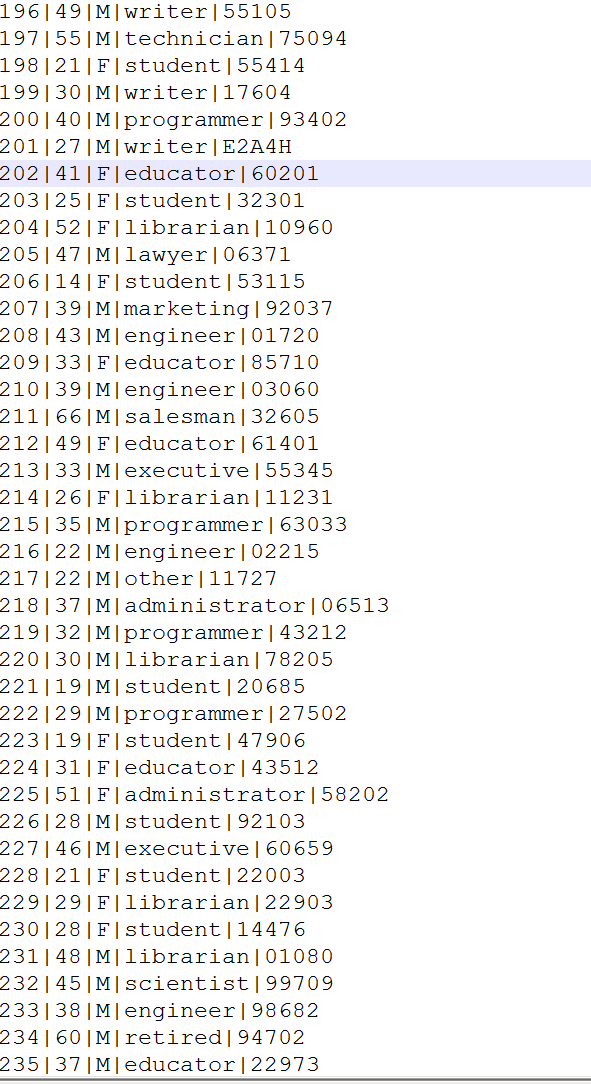
\includegraphics[scale=0.55]{sampleuser.png}
        \caption{Sample list of user data}
        \label{Samplelist1}
    \end{center}
\end{figure}
\newpage
\subsubsection{Sample u.item file}
\begin{figure}[ht]    
    \begin{center}
        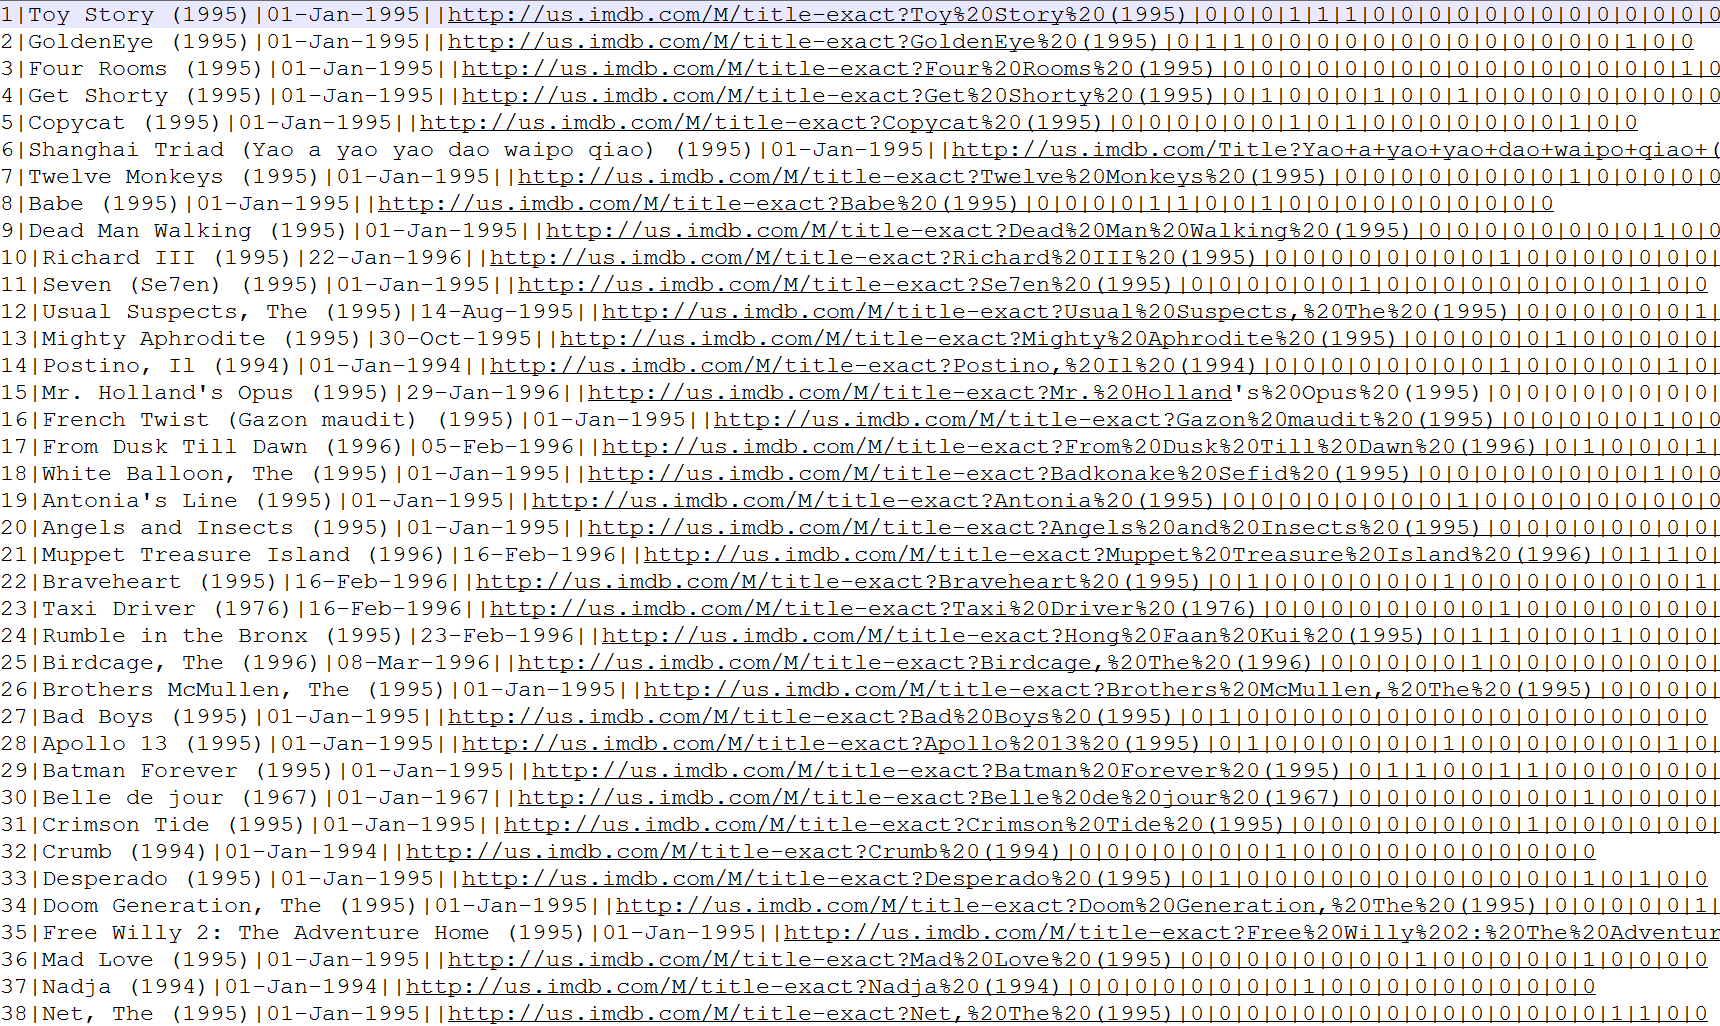
\includegraphics[scale=0.4]{sample_uitem.png}
        \caption{Sample list of movie data}
        \label{Samplelist2}
    \end{center}
\end{figure}
\newpage

\subsubsection{Sample u.data file}
\begin{figure}[ht]    
    \begin{center}
        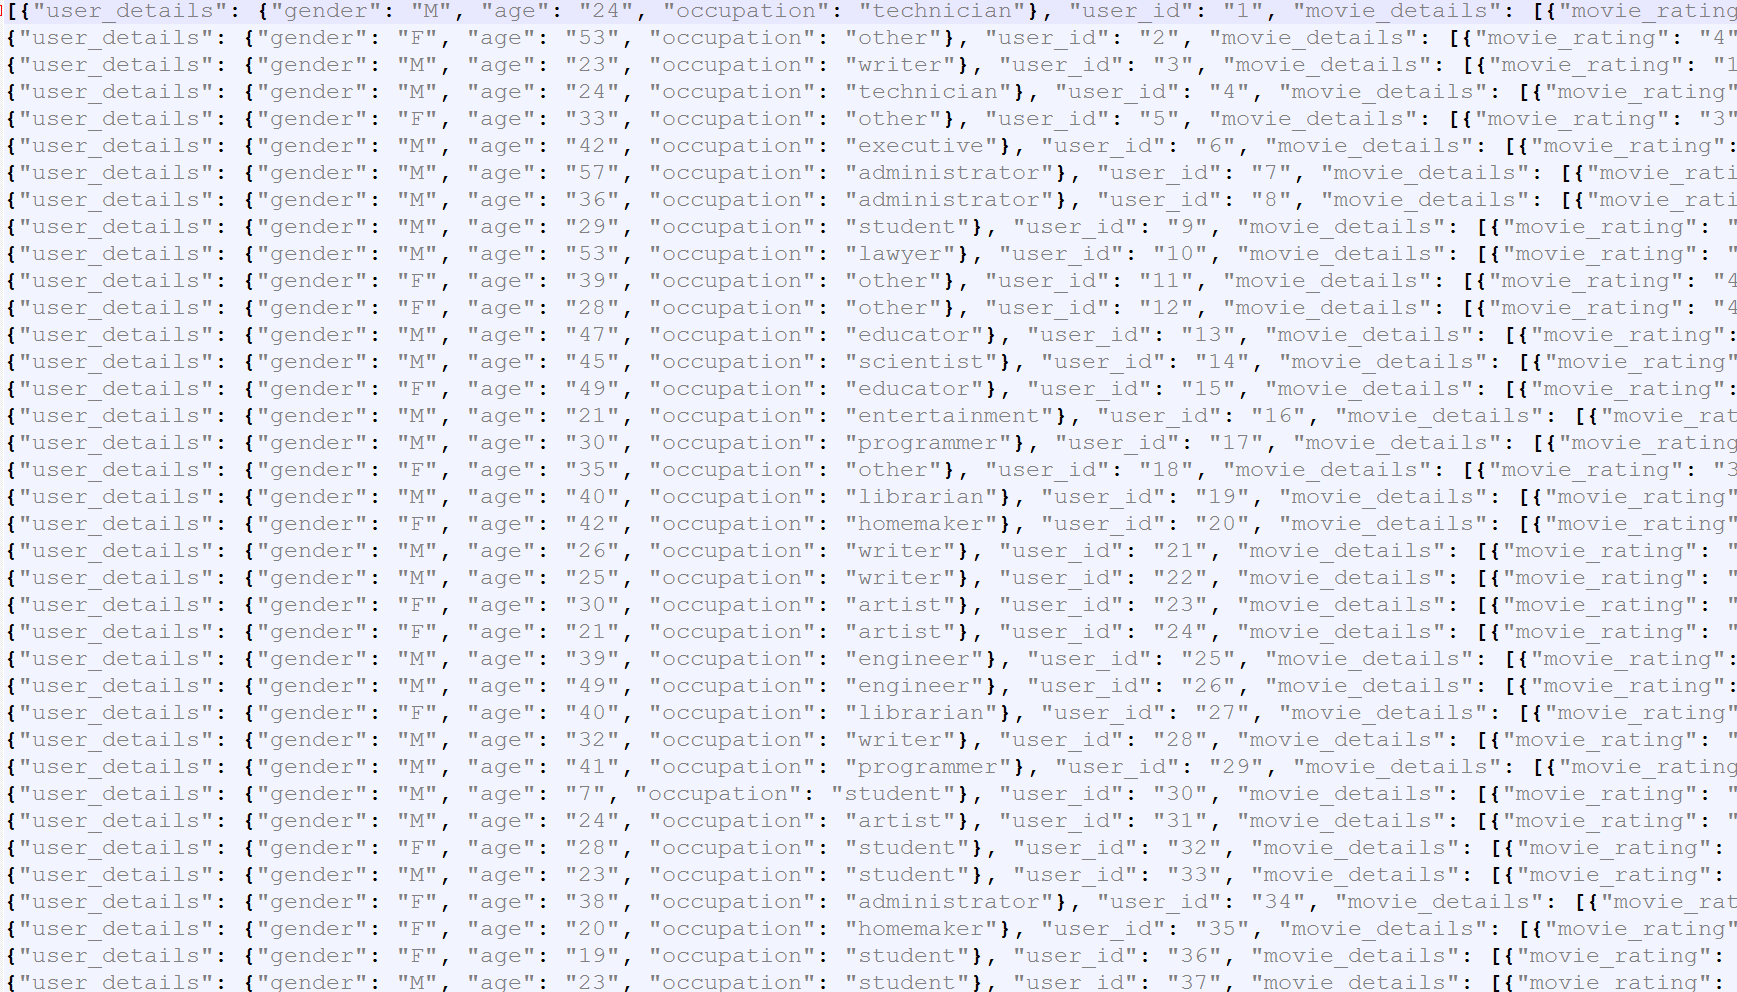
\includegraphics[scale=0.4]{sample_udata.png}
        \caption{Sample list of users and their rating for each movie}
        \label{Samplelist3}
    \end{center}
\end{figure}
\newpage
\subsection{Outputs}

\subsubsection{Sample combined data}
\begin{figure}[ht]    
    \begin{center}
        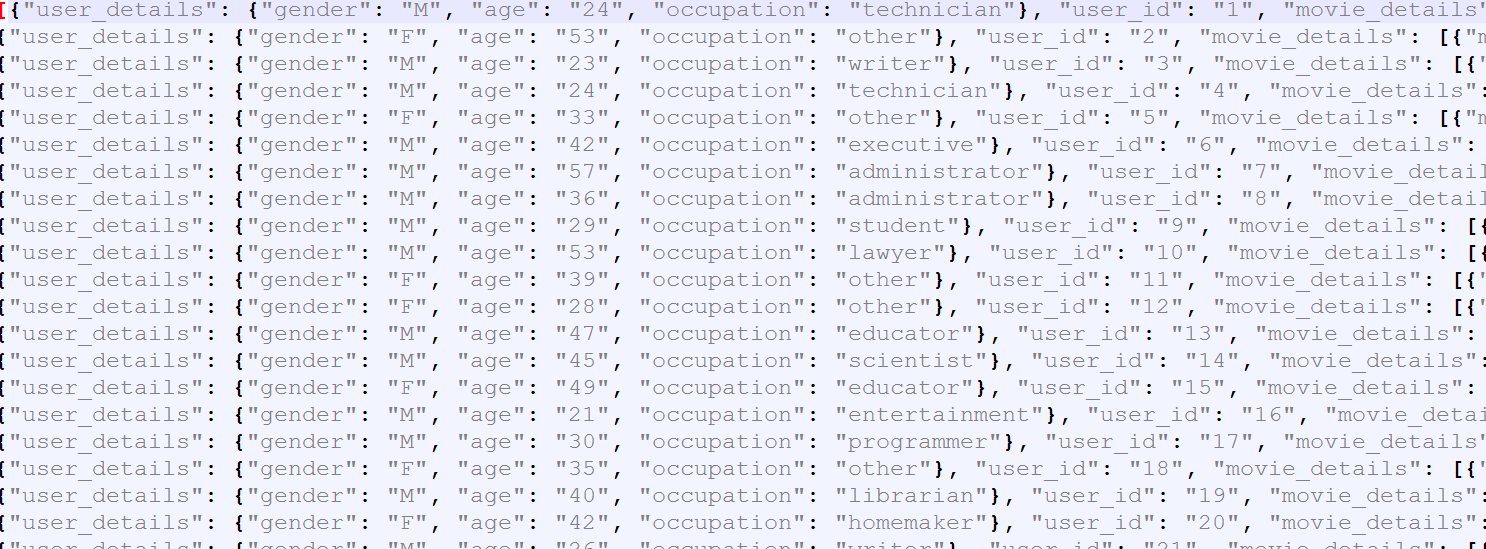
\includegraphics[scale=0.4]{sample_combined.png}
        \caption{Sample data combining all the three data files shown above}
        \label{Samplelist4}
    \end{center}
\end{figure}
\newpage

\subsubsection{Similar users data}
\begin{figure}[ht]    
    \begin{center}
        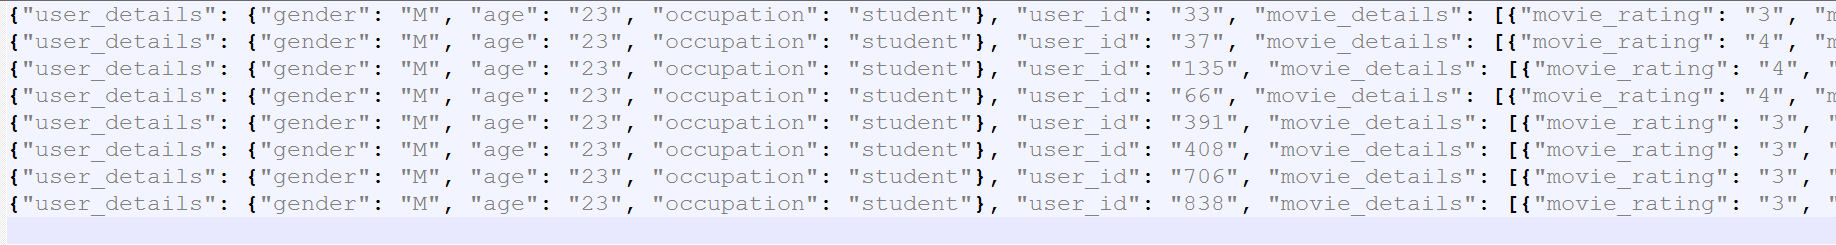
\includegraphics[scale=0.36]{similarusers.png}
        \caption{List of users similar to me in terms of age,gender and occupation}
        \label{Samplelist5}
    \end{center}
\end{figure}
\newpage
\subsubsection{Output file}
\begin{figure}[ht]    
    \begin{center}
        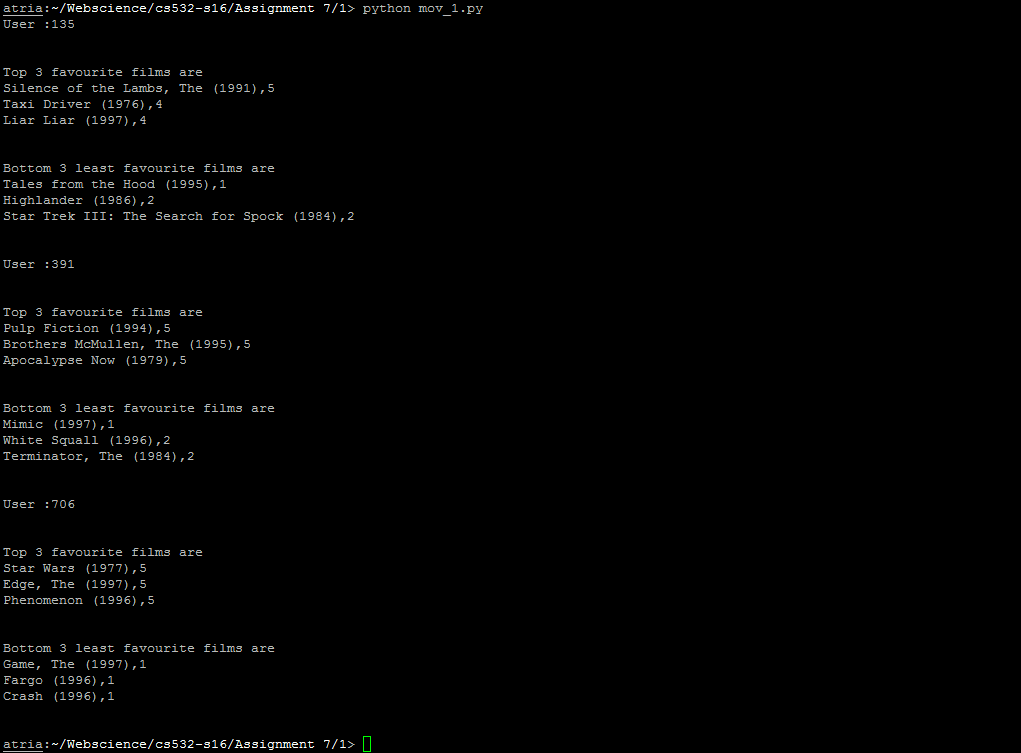
\includegraphics[scale=0.7]{topandbot3.png}
        \caption{File shows 5 top favorite and least favorite movies for each of the 3 users who are closest to me}
        \label{output1}
    \end{center}
\end{figure}
\newpage